% =====================================================================
%  DA-ZVAD -- combined project report, IEEE conference format (IEEEtran)
%  Phase 1 (paper1_concept_shift.tex): CLIP + scene description, its
%  diagnosis and its failure.  Phase 2 (paper2_frozen_normality.tex): the
%  fixed text prior on PE-Core and the sealed UBnormal test.
%  Every number is taken from those two papers; nothing is re-measured.
%
%  Overleaf: upload this file, references.bib and the figure PDFs listed
%  below (flat, or in a figures/ folder). Compiler: pdfLaTeX. Recompile twice.
%  FIGURES: fig_architecture_clip, fig_architecture_final, fig_dataset_samples,
%           fig_camera_baselines, fig_chart_sweep, fig_roc_curves,
%           fig_p2_timeline, fig_p2_progression, fig_p2_forest, fig_p2_dev_roc,
%           fig_p2_ubnormal, fig_p2_ubnormal_types, fig_p2_comparison
% =====================================================================
\documentclass[conference,a4paper]{IEEEtran}

\usepackage{cite}
\usepackage{amsmath,amssymb}
\usepackage{graphicx}
\usepackage{booktabs}
\usepackage{array}
\usepackage{tabularx}
\usepackage{multirow}
% rotating: each architecture diagram sits on its own landscape page, where it
% prints at full size (it is drawn 8.4 in wide; the two-column text block is 7.2 in)
\usepackage{rotating}
\usepackage{algorithm}
\usepackage{algpseudocode}
\usepackage{url}
\graphicspath{{./}{figures/}}

% every chart was drawn 6.9 in wide, so charts span both columns (figure*)
\renewcommand{\topfraction}{0.9}
\renewcommand{\dbltopfraction}{0.9}
\renewcommand{\textfraction}{0.07}
\renewcommand{\floatpagefraction}{0.75}
\renewcommand{\dblfloatpagefraction}{0.75}
\setcounter{topnumber}{3}
\setcounter{dbltopnumber}{2}
\setcounter{totalnumber}{5}

\newcolumntype{Z}{>{\raggedright\arraybackslash}X}
\newcolumntype{W}[1]{>{\raggedright\arraybackslash}p{#1}}
\newcommand{\ci}[2]{\,[{#1},\,{#2}]}

\begin{document}

\title{Training-Free Video Anomaly Detection under Concept Shift:\\
From Per-Camera Scene Descriptions to a Frozen Text Prior\\
Verified by a Sealed Test}

\author{\IEEEauthorblockN{Prakash Kumar Sarangi}
\IEEEauthorblockA{M.Tech, Computer Science and Engineering\\
National Institute of Technology Calicut\\
Kozhikode, Kerala, India}
\and
\IEEEauthorblockN{Dr Pranesh Das and Dr Raju Hazari}
\IEEEauthorblockA{Supervisors, Department of Computer Science and Engineering\\
National Institute of Technology Calicut\\
Kozhikode, Kerala, India}}

\maketitle

% ---------------------------------------------------------------------
\begin{abstract}
Training-free video anomaly detection (VAD) scores frames against text with a
frozen vision-language model, so the text does the work that training used to
do. We first argue that anomaly
detection is dominated by \emph{concept shift}, in which the same input is
labelled differently in different places, and that the domain-adaptation
literature sets this shift aside. Phase~1 builds a fully frozen CLIP ViT-L/14
detector whose only adaptation channel is a one-sentence scene description, written by a frozen LLaVA model from each
camera's first frames. A falsifying control shows that the description is
load-bearing on ShanghaiTech ($0.751$ AUROC with per-camera descriptions) and
UCF-Crime ($0.824$ $[0.756, 0.877]$). However, a pre-specified audit attributes
$82$--$87\%$ of its gains to calibration across cameras, and the description
fails on XD-Violence (average precision $0.624 \to 0.417$) because the opening
frames often already show the violence. Phase~2 replaces per-camera text with
one fixed text prior, scored with a frozen PE-Core encoder: eight calm,
low-motion normal phrases and a frozen bank of 48 concrete actions. We developed
it one change at a time, under rules committed before each step. It reaches
$0.783$, $0.856$, $0.722$ (AP) and $0.639$ on ShanghaiTech, UCF-Crime,
XD-Violence and NWPU Campus, and exceeds the description-based system on
XD-Violence by $+0.305$ $[+0.255, +0.359]$. We then froze the model, the metrics
and the permitted wording of each outcome before obtaining a fifth benchmark.
Scored once on the UBnormal test split, the model reaches a micro AUROC of
$0.747$ $[0.704, 0.789]$, $+0.096$ $[+0.051, +0.142]$ above plain PE-Core, and
all three pre-registered predictions hold.
\end{abstract}

\begin{IEEEkeywords}
video anomaly detection, training-free detection, concept shift, domain
adaptation, vision-language models, prompt design, pre-registration, sealed
evaluation
\end{IEEEkeywords}

% =====================================================================
\section{Introduction}
\label{sec:intro}
% =====================================================================

Anomaly detection identifies rare, unexpected events in images or video. Its
dominant formulation is one-class learning: a model of ``normal'' is estimated
from normal footage, and departures from it are flagged. The learned normality
is bound to the place where it was estimated. A new camera, site or application
therefore needs fresh data and a new training run, and a surveillance network
of hundreds of cameras cannot afford that for each one.

Training-free VAD removes the training run. A frozen vision-language model,
such as CLIP \cite{radford2021clip}, compares each frame with a few sentences,
and nothing is learned at the target site
\cite{zanella2024lavad, anyanomaly2025, yin2026nova, lee2025flashback,
zou2026askhint}. The sentences then do the work that training used to do. The
question this report answers is \emph{what those sentences should say, and who
should write them}.

We approach it in two phases.

\emph{Phase~1: a description of each camera's scene.} The domain-adaptation (DA)
literature concentrates, by an explicit scoping decision, on covariate shift, a
change in the input distribution. In anomaly detection normality depends on
context: the same vehicle is normal on a road and anomalous on a walkway. That is
concept shift, the type the literature sets aside. If a foundation model already
absorbs most covariate shift, a natural response is to tell it in words where it
is. We build a fully frozen detector in which a scene description is the only
quantity that varies, so its effect is identifiable. We test it with a protocol
whose deliberately wrong description could refute the claim. The description
turns out to be load-bearing but fragile. Most of its benefit is calibration,
which moves each camera's scores up or down as a block. On XD-Violence it fails
outright, because the frames it is written from often already show the event.

\emph{Phase~2: one fixed text prior for every camera.} The lesson of Phase~1 is
that text derived from a camera's own footage inherits whatever that footage
shows. Phase~2 therefore fixes one text prior for all cameras: a description of
what calm, ordinary footage looks like, and a list of concrete things that go
wrong. A fixed list is easy to over-fit to the benchmarks used to write it, so we
separated development from testing as strictly as we could. Every change was made
one at a time, under rules committed before it was scored. When development
ended, the model, the evaluation and the wording permitted for each outcome were
frozen. Only then was a fifth benchmark, UBnormal \cite{acsintoae2022ubnormal},
downloaded and scored, once.

\paragraph*{Contributions}
\begin{enumerate}
  \item \textbf{Characterisation.} We state concept shift as the dominant form of
        domain shift in VAD, in the DA literature's own vocabulary
        (Section~\ref{sec:gap}).
  \item \textbf{An identifiable mechanism and a falsifiable protocol.} A fully
        frozen pipeline with a four-condition context sweep. The sweep shows
        that \emph{where} a description enters the prompts matters more than
        what it says: adding it to both ensembles reverses its effect
        (Section~\ref{sec:p1-results}).
  \item \textbf{What a scene description does, and where it fails.} Between
        $82\%$ and $87\%$ of its gains are calibration, and it fails when it is
        written from frames that already show the anomaly
        (Sections~\ref{sec:p1-audit}--\ref{sec:p1-fail}).
  \item \textbf{A camera-agnostic text prior.} Eight calm normal phrases,
        following the normality rules of NOVA \cite{yin2026nova}, and a frozen
        bank of 48 concrete actions, used unchanged on every camera with a frozen
        PE-Core encoder \cite{bolya2025pe}. The calm phrases help PE-Core but not
        CLIP, and on two benchmarks they re-rank frames within a video
        (Section~\ref{sec:p2-results}).
  \item \textbf{A sealed test.} A complete evidence chain, from committed rules
        to one scored run on a benchmark obtained after freezing
        (Section~\ref{sec:sealed}).
  \item \textbf{A record of what failed}, reported with its numbers in both
        phases.
\end{enumerate}

% =====================================================================
\section{Related Work}
\label{sec:related}
% =====================================================================

\subsection{Domain adaptation}
Domain adaptation keeps the task fixed while the data distribution changes.
Patel et~al.\ \cite{patel2015visual} review the shallow era: subspace
alignment, geodesic-flow interpolation and shared latent spaces. Wang and
Deng \cite{wang2018deep} divide deep DA into discrepancy-based,
adversarial-based and reconstruction-based methods. Wilson and Cook
\cite{wilson2020survey} organise unsupervised DA by mechanism, alongside the
generalisation bound that motivates divergence minimisation. Liu
et~al.\ \cite{liu2022deep} survey modern unsupervised DA and restrict
themselves explicitly to covariate shift. Singhal et~al.\ \cite{singhal2023domain}
list covariate shift as a theoretical condition for DA. For large language
models, Fan et~al.\ \cite{fan2026llm} describe adaptation as a continuum from
prompt engineering to fine-tuning. At the prompt end of that continuum the model
is unchanged and the \emph{input context} carries the adaptation, a category the
visual taxonomies do not contain. Within VAD, Ada-VAD \cite{adavad2024} adapts
adversarially to a few target frames, Lu et~al.\ \cite{lu2020fewshot}
meta-learn scene adaptation, and zxVAD \cite{aich2023zxvad} transfers without
any target adaptation. All of them still train on source data, and none lets an
operator \emph{state} what normality means at the target.

\subsection{Training-free video anomaly detection}
WinCLIP \cite{jeong2023winclip} scores images against normal and abnormal
prompt ensembles, and AnomalyCLIP \cite{zhou2024anomalyclip} learns
object-agnostic prompts. In video, LAVAD \cite{zanella2024lavad} captions every
frame and asks a large language model to score the captions. AnyAnomaly
\cite{anyanomaly2025} lets the user name the anomaly and queries a large
vision-language model several times per segment. VERA \cite{ye2025vera} learns
verbal guiding questions on training data. NOVA \cite{yin2026nova} strengthens
the normal side. It keeps anomaly-adjacent verbs out of normal prompts, biases
normal descriptions toward static, low-motion scenes, and adds a visual normal
anchor built from each test video's initial frames. ASK-Hint
\cite{zou2026askhint} poses action-centric guiding questions to a frozen
vision-language model. Flashback \cite{lee2025flashback} builds a memory of
generated captions offline and needs no language model at inference. Song and
Lee \cite{song2026vlmanswer} show that a model's yes/no answer is a poor ranking
score unless its probabilities are used. Table~\ref{tbl:position} places these
methods by what their text requires, and
Tables~\ref{tbl:lit-da}--\ref{tbl:lit-vad} summarise the literature reviewed.

\begin{table}[!t]
\caption{Training-free detectors by the text they use. ``Target video'': the
text or normal reference is derived from the video being scored. ``LLM at
test'': a language or vision-language model is queried during detection.}
\label{tbl:position}
\centering
\footnotesize
\begin{tabularx}{\columnwidth}{@{}l Z c c@{}}
\toprule
\textbf{Method} & \textbf{Text and normal reference} & \textbf{Target video} & \textbf{LLM at test} \\
\midrule
LAVAD \cite{zanella2024lavad} & captions of the video's frames, scored by an LLM & yes & yes \\
AnyAnomaly \cite{anyanomaly2025} & anomaly named by the user & no & yes \\
NOVA \cite{yin2026nova} & low-motion normal prompts; visual anchor from each video's first frames & yes & no \\
ASK-Hint \cite{zou2026askhint} & guiding questions grouped by anomaly category & no & yes \\
Flashback \cite{lee2025flashback} & memory of generated captions, built offline & no & no \\
\textbf{Phase 1 (ours)} & a caption of each camera's first frames & yes & no \\
\textbf{Phase 2 (ours)} & \textbf{59 fixed phrases, the same for every camera} & \textbf{no} & \textbf{no} \\
\bottomrule
\end{tabularx}
\end{table}

\begin{table*}[!t]
\caption{Domain-adaptation literature reviewed, with the challenge and future
scope each leaves for a training-free detector that must adapt without target
data.}
\label{tbl:lit-da}
\centering
\footnotesize
\begin{tabularx}{\textwidth}{@{}W{2.6cm} l W{2.3cm} Z Z Z@{}}
\toprule
\textbf{Work} & \textbf{Year} & \textbf{Venue} & \textbf{Key idea} & \textbf{Challenge / limitation} & \textbf{Future scope} \\
\midrule
Patel et al.\ \cite{patel2015visual} & 2015 & IEEE Signal Process.\ Mag. & Survey of shallow visual DA: subspace alignment, geodesic flow, dictionary learning & Hand-crafted features; target data needed; one labelling function assumed & Deep, label-efficient adaptation \\
Wang and Deng \cite{wang2018deep} & 2018 & Neurocomputing & Deep DA taxonomy: discrepancy, adversarial and reconstruction methods & Every family trains on target samples; aligns $p(x)$ only & Adaptation without target training \\
Kouw and Loog \cite{kouw2018introduction} & 2018 & arXiv & Formal taxonomy of shift: covariate, conditional, label, concept & Concept shift defined but left largely without methods & Methods for shift in $p(y\mid x)$ \\
Wilson and Cook \cite{wilson2020survey} & 2020 & ACM Comput.\ Surv. & Unsupervised deep DA by mechanism; the generalisation bound & The bound presumes a shared labelling function & Settings where that fails \\
Liu et al.\ \cite{liu2022deep} & 2022 & APSIPA Trans. & Modern unsupervised DA: alignment, adversarial, generative, self-training & Scope restricted to covariate shift & Source-free, test-time and foundation-model DA \\
Singhal et al.\ \cite{singhal2023domain} & 2023 & IEEE Access & Theory and settings of DA (closed, partial, open-set, universal) & Lists covariate shift as a condition for DA & Adaptation when it is violated \\
Fan et al.\ \cite{fan2026llm} & 2026 & Solid Earth Sci. & LLM adaptation as a cost--performance continuum, prompting to fine-tuning & Prompting cheapest but ``often lacks depth and robustness'' & Prompt-level adaptation for vision \\
Wilkinghoff et al.\ \cite{wilkinghoff2026context} & 2026 & arXiv & Position: normality depends on operating context & No method; context from extra sensors & Conditional assessment, measured \\
Lu et al.\ \cite{lu2020fewshot} & 2020 & ECCV & Meta-learned scene adaptation from a few frames & Needs target frames and an update & Adaptation with no update \\
zxVAD \cite{aich2023zxvad} & 2023 & WACV & Cross-domain VAD with pseudo-anomalies, no target adaptation & Normality fixed by source statistics & Operator-specified normality \\
Ada-VAD \cite{adavad2024} & 2024 & SDM & Domain-invariant predictor adapted adversarially to target frames & A training run per deployment & Training-free adaptation \\
\bottomrule
\end{tabularx}
\end{table*}

\begin{table*}[!t]
\caption{Anomaly-detection literature reviewed, in order of year.}
\label{tbl:lit-vad}
\centering
\footnotesize
\begin{tabularx}{\textwidth}{@{}W{2.6cm} l W{1.3cm} Z Z Z@{}}
\toprule
\textbf{Work} & \textbf{Year} & \textbf{Venue} & \textbf{Key idea} & \textbf{Challenge / limitation} & \textbf{Future scope} \\
\midrule
CLIP \cite{radford2021clip} & 2021 & ICML & Contrastive image--text pre-training; zero-shot classification from text & One embedding per image at $224\times224$; small objects lost & Region- and patch-level use \\
WinCLIP \cite{jeong2023winclip} & 2023 & CVPR & Zero-shot anomaly detection with prompt ensembles and windows & Industrial images; normality not tied to a scene & Video, scene-dependent normality \\
AnomalyCLIP \cite{zhou2024anomalyclip} & 2024 & ICLR & Learned object-agnostic prompts & Needs auxiliary labelled data & Fully training-free prompting \\
LAVAD \cite{zanella2024lavad} & 2024 & CVPR & Frame captions scored by an LLM, refined by cross-modal similarity & Chains captioner, LLM and refiner; context not isolated & Lighter scoring; role of context \\
OVVAD \cite{wu2024ovvad} & 2024 & CVPR & Open-vocabulary VAD with frozen CLIP and trained heads & Heads trained on the benchmark & Zero-shot transfer \\
AnomalyRuler \cite{yang2024anomalyruler} & 2024 & arXiv & An LLM induces rules of normality from a few normal frames & Needs target frames and GPT-4 & Rules without target frames \\
VERA \cite{ye2025vera} & 2025 & CVPR & Frozen VLM guided by verbal questions learned on training data & Questions optimised offline on labelled data & Explanations under shift \\
Flashback \cite{lee2025flashback} & 2025 & arXiv & Retrieval from a memory of generated captions & Deployment scene not isolated & Scene-aware memories \\
AnyAnomaly \cite{anyanomaly2025} & 2026 & WACV & The user names the anomaly; three large-VLM queries per segment & Classes named in advance; heavy inference & Unnamed anomalies \\
ASK-Hint \cite{zou2026askhint} & 2026 & WACV & Action-centric, fine-grained prompts for frozen VLMs & Deployment scene not isolated & Scene-conditioned prompting \\
NOVA \cite{yin2026nova} & 2026 & arXiv & Prompt banks per anomaly class; calm normal prompts; visual anchor & Banks per class; anchor from each test video & Normal side without class lists \\
Song and Lee \cite{song2026vlmanswer} & 2026 & arXiv & A VLM's yes/no answer is not an anomaly score & Score design, not adaptation & Rank-preserving scores \\
PE-Core \cite{bolya2025pe} & 2025 & arXiv & Perception Encoder: a stronger contrastive image--text model & Best features inside the network & Use as a frozen VAD encoder \\
\bottomrule
\end{tabularx}
\end{table*}

% =====================================================================
\section{Concept Shift and the Research Gap}
\label{sec:gap}
% =====================================================================

A domain is a joint distribution $P(x,y)=P(y\mid x)\,P(x)$, and shift may occur
in any factor (Table~\ref{tbl:shifts}). Liu et~al.\ \cite{liu2022deep} state that
concept shift ``is, however, usually not a common problem in popular object
classification or semantic segmentation tasks'' and focus on covariate shift.
Singhal et~al.\ \cite{singhal2023domain} give $P(Y_s\mid X_s)=Q(Y_t\mid X_t)$ as a
condition under which DA is justified; classical theory thus \emph{assumes
concept shift away}.

\begin{table}[!t]
\caption{The four types of domain shift, and concept shift in VAD.}
\label{tbl:shifts}
\centering
\footnotesize
\begin{tabularx}{\columnwidth}{@{}l l Z@{}}
\toprule
\textbf{Shift} & \textbf{Factor} & \textbf{Example} \\
\midrule
Covariate & $p(x)$ & Same objects, different camera or lighting \\
Conditional & $p(x\mid y)$ & A class looks different across domains \\
Label & $p(y)$ & Class proportions differ \\
\textbf{Concept} & $p(y\mid x)$ & \textbf{Same input, different label} \\
\midrule
\multicolumn{3}{@{}l}{\emph{Concept shift in VAD: same content, label inverts}} \\
A person running & $p(y\mid x)$ & park: normal; bank vault: anomalous \\
A person lying down & $p(y\mid x)$ & beach: normal; factory aisle: anomalous \\
A vehicle & $p(y\mid x)$ & road: normal; walkway: anomalous \\
\bottomrule
\end{tabularx}
\end{table}

In anomaly detection, normality belongs to the deployment context and not to the
object, so the label can invert while $p(x)$ stays the same. Methods that align
$p(x)$ are the wrong instrument for that. Liu et~al.\ \cite{liu2022deep} also
note that foundation models ``are robust to the covariate shift in many cases''.
A frozen CLIP encoder has seen an enormous variety of cameras and lighting, so
the shift that remains is the one the literature excluded. Wilkinghoff
et~al.\ \cite{wilkinghoff2026context} independently argue that normality is
context-dependent, in a position paper with context drawn from extra sensors. We
supply instead a mechanism, context given as text, and a protocol that measures
it.

\paragraph*{Research gaps}
\begin{description}
  \item[G1.] Concept shift dominates VAD but has not been studied as such in DA
        terms.
  \item[G2.] No protocol measures whether a \emph{description} adapted anything.
  \item[G3.] Little is known empirically about which shifts a frozen
        vision-language model absorbs unaided.
  \item[G4.] Training-free detectors are chosen and reported on the same test
        videos; none reports a benchmark held out from its own design.
\end{description}

\paragraph*{Formulation}
Two deployment domains $\mathcal{D}_A$ and $\mathcal{D}_B$ exhibit concept shift
when
\begin{equation}
p_A(x)\approx p_B(x) \qquad\text{while}\qquad p_A(y\mid x)\neq p_B(y\mid x).
\label{eq:conceptshift}
\end{equation}
We score with text $c$ and a model whose parameters $\theta$ are all frozen,
\begin{equation}
s(x\mid c) = f_\theta(x, c), \qquad \theta\ \text{fixed}.
\label{eq:score}
\end{equation}
Because $\theta$ cannot change, any difference between $s(x\mid c_A)$ and
$s(x\mid c_B)$ is attributable to the text alone. In Phase~1, $c$ is a
description of each camera's scene; in Phase~2 it is one fixed text prior
shared by every camera.

\paragraph*{Research questions}
\begin{description}
  \item[RQ1.] Is a scene description load-bearing: does a wrong one cost accuracy?
  \item[RQ2.] What decides whether it helps: wording, point of injection, or the
        number of scenes?
  \item[RQ3.] Does it re-rank frames within a video, or calibrate videos against
        one another?
  \item[RQ4.] Where does it fail, and can a fixed text prior, with no input from
        the camera, do better on a benchmark held out from its design?
\end{description}

% =====================================================================
\section{Phase 1: DA-ZVAD with a Scene Description}
\label{sec:p1-method}
% =====================================================================

\subsection{Pipeline}
DA-ZVAD is an inference pipeline of four frozen modules
(Fig.~\ref{fig:arch1}), run in five stages; Algorithm~\ref{alg:infer} gives the
procedure.

\begin{sidewaysfigure*}
\centering
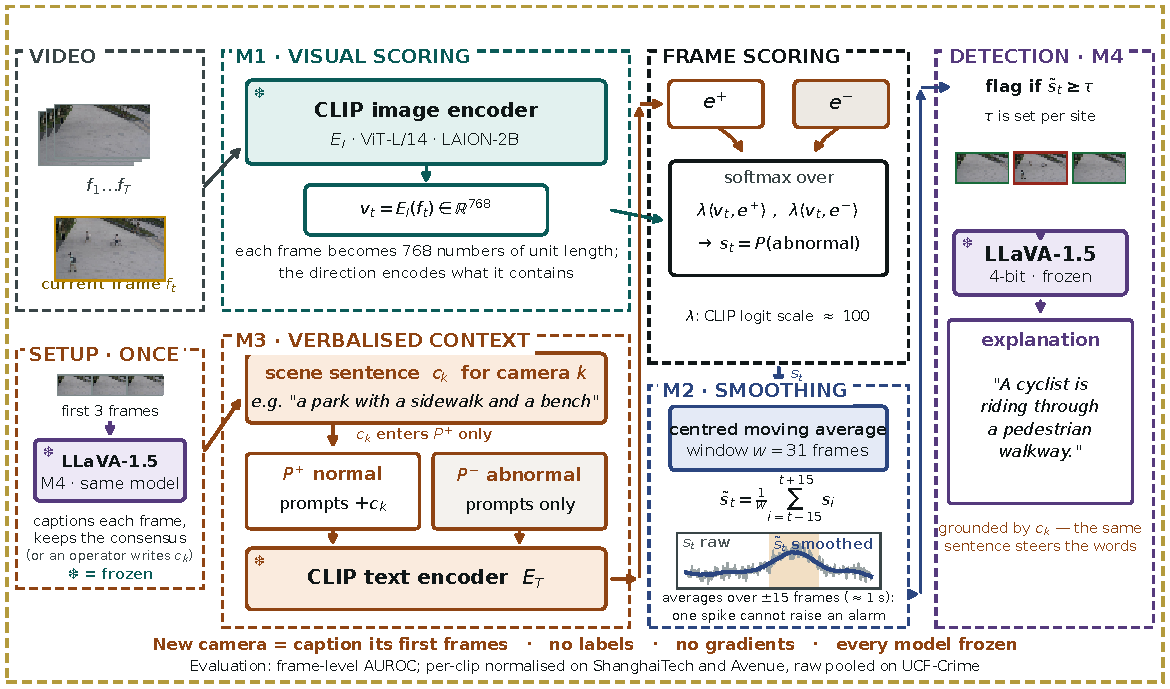
\includegraphics[width=0.95\textheight]{fig_architecture_clip}
\caption{Phase~1: the DA-ZVAD framework. Every model is frozen; the verbalised
scene context (M3) is the only adaptation mechanism. At setup, the frozen LLaVA
model captions a camera's first three frames, and the consensus caption becomes
that camera's descriptor $c_k$, so no human-written text is needed. $c_k$ enters
the normal prompt ensemble only, and also grounds the generated
explanations.}\label{fig:arch1}
\end{sidewaysfigure*}

\begin{description}
  \item[M1 Visual encoder.] A frozen CLIP ViT-L/14 \cite{radford2021clip,
        dosovitskiy2021vit} embeds each sampled frame as a unit vector $v_t$.
  \item[M2 Temporal aggregation.] A centred moving average of width $w$.
  \item[M3 Verbalised context.] The scene description $c$ is appended to the
        \emph{normal} prompt ensemble only.
  \item[M4 Reasoning.] A frozen LLaVA-1.5-7B \cite{liu2023llava} in 4-bit
        \cite{dettmers2023qlora}. At installation it captions the first three
        sampled frames of a camera under the instruction ``Describe only the
        location and its layout \ldots\ Do not mention people''. In operation it
        explains each detected event.
\end{description}

The normal ensemble $P^{+}$ holds three phrases (``a normal day with people
behaving ordinarily'', ``a calm and safe public area'', ``nothing dangerous or
abnormal is happening''), and the abnormal ensemble $P^{-}$ three more (``a
dangerous or violent event'', ``a fight, robbery or accident in progress'', ``an
abnormal and unsafe situation''). M3 adds ``$c$, everything is normal'' and
``$c$, a usual and safe moment'' to $P^{+}$. For ShanghaiTech camera~01 the
generated $c$ is ``a paved walkway with a bench and a tree''. Each ensemble is
encoded, averaged and renormalised into a prototype $e^{\pm}$, and each frame
scores
\begin{equation}
s_t = \frac{\exp(\lambda\langle v_t, e^{-}\rangle)}
{\exp(\lambda\langle v_t, e^{+}\rangle)+\exp(\lambda\langle v_t, e^{-}\rangle)}
= \sigma\big(\lambda(\langle v_t,e^{-}\rangle-\langle v_t,e^{+}\rangle)\big),
\label{eq:framescore}
\end{equation}
with $\lambda=100$, CLIP's learned logit scale. The scores are then smoothed,
\begin{equation}
\tilde{s}_t=\frac{1}{|\mathcal{W}_t|}\sum_{k\in\mathcal{W}_t}s_k,\qquad
\mathcal{W}_t=[t-\lfloor w/2\rfloor,\,t+\lfloor w/2\rfloor]\cap[1,T].
\label{eq:smooth}
\end{equation}
Every second frame is scored on ShanghaiTech and CUHK Avenue ($w=31$), and every
sixteenth elsewhere ($w=5$). Both windows span roughly two to three seconds. The
pipeline fits in about 7\,GB of GPU memory.

\begin{algorithm}[!t]
\caption{DA-ZVAD inference for one video}
\label{alg:infer}
\begin{algorithmic}[1]
\Require frames $x_{1..T}$; text $c$; window $w$; threshold $\tau$
\State $(P^{+},P^{-})\gets\textproc{Prompts}(c)$ \Comment{Phase 1: $c$ into $P^{+}$}
\State $e^{\pm}\gets\textproc{MeanPool}(E_{\text{text}}(P^{\pm}))$
\For{$t=1$ \textbf{to} $T$}
  \State $v_t\gets E_{\text{img}}(x_t)$
  \State $s_t\gets\sigma(\lambda(\langle v_t,e^{-}\rangle-\langle v_t,e^{+}\rangle))$
\EndFor
\State $\tilde{s}\gets\textproc{MovingAverage}(s,w)$
\State events $\gets$ runs of $\tilde{s}_t\ge\tau$; explain each peak frame
\State \Return $\tilde{s}$, events
\end{algorithmic}
\end{algorithm}

\subsection{The context sweep}
\label{sec:sweep}
The pipeline is run repeatedly on identical data with everything fixed except
$c$, under four conditions (Table~\ref{tbl:variants}). If the adaptation claim
holds, the expected order is matched $\gtrsim$ generic $\gtrsim$ none, with
mismatched clearly \emph{worse}. A detector that ignored its text would show no
difference, which would refute the claim.

\begin{table}[!t]
\caption{The four conditions of the context sweep. Only the text differs.}
\label{tbl:variants}
\centering
\footnotesize
\begin{tabularx}{\columnwidth}{@{}l Z Z@{}}
\toprule
\textbf{Condition} & \textbf{Descriptor} & \textbf{Purpose} \\
\midrule
none & M3 disabled & Lower reference \\
generic & ``a generic scene'' & Presence of any text \\
matched & correct description & Proposed operating condition \\
mismatched & wrong domain (industrial text on surveillance data) & \textbf{Falsifying control} \\
\bottomrule
\end{tabularx}
\end{table}

% =====================================================================
\section{Phase 2: A Frozen, Camera-Agnostic Text Prior}
\label{sec:p2-method}
% =====================================================================

\subsection{From lessons to requirements}
Phase~1 (Section~\ref{sec:p1-results}) left four lessons. Each becomes a
requirement for Phase~2.
\begin{description}
  \item[L1.] Text written from a camera's opening frames inherits whatever those
        frames show (the XD-Violence failure).
  \item[L2.] The point at which text enters matters more than its wording.
  \item[L3.] A description mostly calibrates: $82$--$87\%$ of its gains are level
        shifts.
  \item[L4.] A wrong description is worse than none.
\end{description}
\begin{description}
  \item[R1.] \emph{No dependence on the target's footage} (L1, L4): the text is
        written once and is identical for every camera.
  \item[R2.] \emph{Separate sides} (L2): normal and abnormal phrases share no
        wording.
  \item[R3.] \emph{Ranking, not only calibration} (L3): the text should order
        frames within a video.
  \item[R4.] \emph{No model at test time}: one image-encoder pass per frame.
\end{description}

\subsection{Model}
Figure~\ref{fig:arch2} shows the final model, DA-ZVAD~v2. The encoder is
PE-Core-L/14 at $336\times336$ pixels \cite{bolya2025pe}, frozen and used through
\texttt{open\_clip} ($v_t\in\mathbb{R}^{1024}$, logit scale $99.9$; we keep
$\lambda=100$). The scoring rule is unchanged from
Equations~\eqref{eq:framescore} and~\eqref{eq:smooth}, with the prototypes
\begin{equation}
e^{\pm}=\frac{\sum_{p\in P^{\pm}}u(p)}{\big\|\sum_{p\in P^{\pm}}u(p)\big\|}.
\label{eq:proto}
\end{equation}

\begin{sidewaysfigure*}
\centering
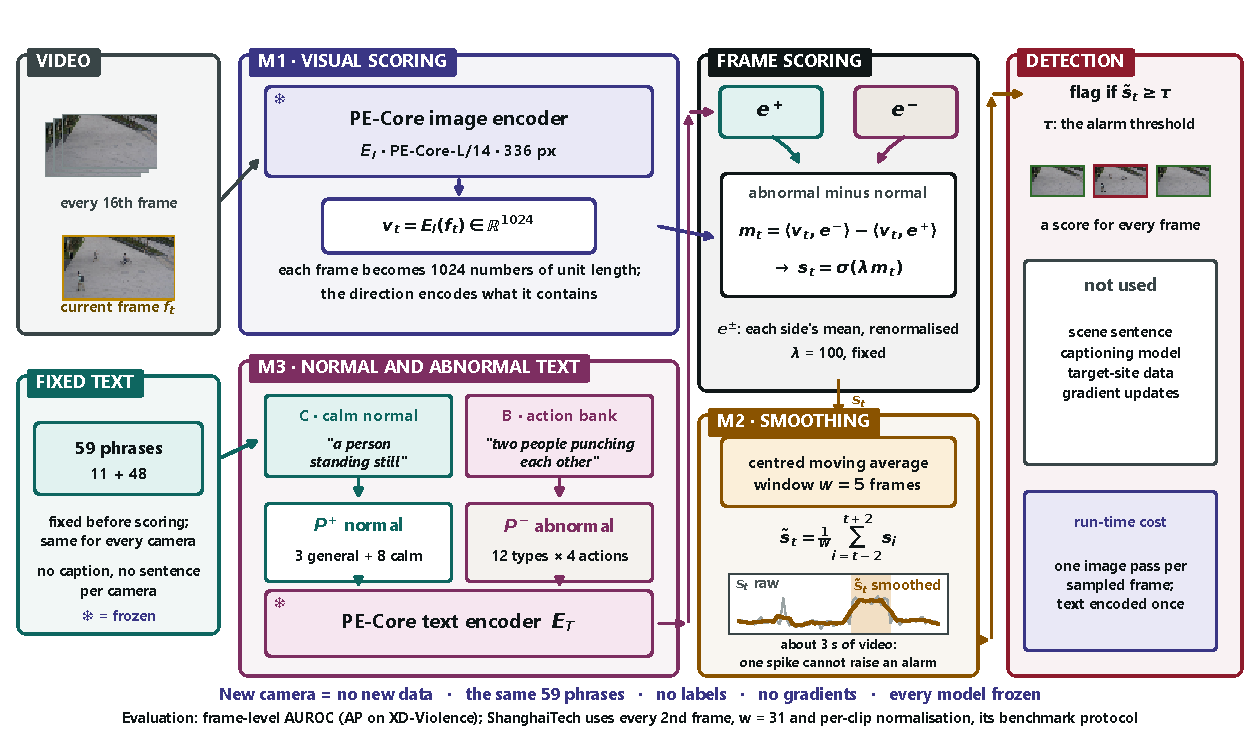
\includegraphics[width=0.95\textheight]{fig_architecture_final}
\caption{Phase~2: DA-ZVAD~v2. M1: a frozen PE-Core image encoder at
$336\times336$ pixels. M3: the normal ensemble (three general phrases and eight
calm phrases, C) and the abnormal ensemble (48 concrete actions in twelve types,
B), embedded once by the frozen text encoder. Frame scoring: the margin between
the two prototypes, passed through a sigmoid. M2: a centred moving average. The
right-hand panel lists what the model does not use.}\label{fig:arch2}
\end{sidewaysfigure*}

\emph{Normal side: calm, low-motion phrases (C).} $P^{+}$ keeps the three general
phrases of Phase~1 and adds eight calm phrases (Table~\ref{tbl:normal}). They
follow the two rules of NOVA's normality-aware prompts \cite{yin2026nova}: no
normal phrase names or resembles an anomalous action, and normal phrases describe
static, low-motion scenes. The phrases are our own. We omit NOVA's visual anchor,
which is computed from each test video's initial frames. A second wording that
shares no phrase with the first is used only as a robustness check.

\begin{table}[!t]
\caption{The normal ensemble $P^{+}$ of DA-ZVAD~v2.}
\label{tbl:normal}
\centering
\footnotesize
\begin{tabularx}{\columnwidth}{@{}l Z@{}}
\toprule
\textbf{Group} & \textbf{Phrases} \\
\midrule
General (3) & a normal day with people behaving ordinarily; a calm and safe public area; nothing dangerous or abnormal is happening \\
Quiet places (4) & an empty walkway; an empty street; an empty room; a quiet open area with nobody around \\
Calm people (4) & a person standing still; a person sitting quietly; two people talking calmly; a person walking slowly \\
\bottomrule
\end{tabularx}
\end{table}

\emph{Abnormal side: a frozen bank of concrete actions (B).} $P^{-}$ replaces the
three abstract phrases with 48 concrete actions, four for each of twelve types
(Table~\ref{tbl:bank}). This follows the finding of ASK-Hint that frozen models
judge actions better than labels \cite{zou2026askhint}. A large language model
wrote the bank once. It was read, committed and frozen before it was first
scored, and it was never edited after a score had been seen.

\begin{table*}[!t]
\caption{The abnormal ensemble $P^{-}$: twelve types, four concrete actions each.
Fixed before first use and identical for every camera and every benchmark.}
\label{tbl:bank}
\centering
\footnotesize
\begin{tabularx}{\textwidth}{@{}W{3.1cm} Z@{}}
\toprule
\textbf{Type} & \textbf{Phrases} \\
\midrule
Fighting & two people punching each other; a person kicking someone on the ground; a group of people brawling; a person violently shoving another person \\
Weapon & a person pointing a gun at someone; a person firing a gun; a person threatening someone with a knife; a person stabbing someone \\
Theft & a person snatching a bag from someone; a robber holding up a cashier; a person stealing goods from a shop; a burglar climbing through a window \\
Vandalism & a person smashing a window; a person kicking a door open; a person damaging a parked car; a person spraying graffiti on a wall \\
Road accident & two cars crashing into each other; a car hitting a pedestrian; a motorcycle skidding across the road; a vehicle overturned on the road \\
Fire or explosion & flames and thick smoke rising from a building; a car on fire; an explosion with debris flying; a blast throwing people to the ground \\
Riot or arrest & a crowd of rioters throwing objects; a mob clashing with police; police wrestling a person to the ground; a person being handcuffed and arrested \\
Abuse & an adult hitting a child; a person dragging another person by force; a person being beaten while lying down; a person being grabbed and restrained \\
Falling & a person collapsing to the ground; a person lying motionless on the ground; a person falling from a height; a person tripping and falling hard \\
Vehicle among pedestrians & a cyclist riding through a crowd of pedestrians; a car driving on a pedestrian walkway; a motorbike riding on a footpath; a person on a skateboard weaving between pedestrians \\
Sudden running & a person sprinting through a crowd; a person chasing someone; people running away in panic; a person jumping over a barrier \\
Trespass & a person climbing over a fence; a person forcing entry into a restricted area; a person leaving a suspicious bag behind; a person hiding and watching people \\
\bottomrule
\end{tabularx}
\end{table*}

\emph{What the model does not use.} No captioning or language model, no
description of the site, no frames or labels from the target benchmark, and no
gradient update. The 59 phrases are encoded once. A new camera is connected and
scored with no input beyond its video.

% =====================================================================
\section{Experimental Setup}
\label{sec:setup}
% =====================================================================

\subsection{Datasets}
Table~\ref{tbl:datasets} lists the benchmarks and Fig.~\ref{fig:samples} shows
example frames. Only official test splits are used; no training video of any
benchmark is touched.

\begin{table*}[!t]
\caption{Datasets, the phase in which each is used, and its protocol. UBnormal
was obtained only after the Phase~2 model was frozen.}
\label{tbl:datasets}
\centering
\footnotesize
\begin{tabularx}{\textwidth}{@{}l l Z l l@{}}
\toprule
\textbf{Dataset} & \textbf{Use} & \textbf{Test split} & \textbf{Metric} & \textbf{Sampling} \\
\midrule
MVTec AD \cite{bergmann2019mvtec} & Phase 1 image baseline & 15 categories, 1{,}725 images, pixel masks & image AUROC & --- \\
CUHK Avenue \cite{lu2013avenue} & Phase 1 & 21 videos, one camera view, 15{,}324 frames & AUROC, per clip normalised & every 2nd, $w{=}31$ \\
ShanghaiTech \cite{liu2018shanghaitech} & Phases 1 and 2 & 107 clips, 12 campus cameras, 40{,}791 frames & AUROC, per clip normalised & every 2nd, $w{=}31$ \\
UCF-Crime \cite{sultani2018ucfcrime} & Phases 1 and 2 & 290 videos (140 anomalous), real CCTV, 13 crime classes & AUROC & every 16th, $w{=}5$ \\
XD-Violence \cite{wu2020xdviolence} & Phases 1 and 2 & 800 videos (500 violent): films, sport, news, CCTV & AP & every 16th, $w{=}5$ \\
NWPU Campus \cite{cao2023nwpu} & Phases 1 and 2 & 242 videos, 43 scenes, scene-dependent anomalies & AUROC & every 16th, $w{=}5$ \\
\midrule
UBnormal \cite{acsintoae2022ubnormal} & \textbf{sealed test} & 211 videos (158 abnormal), 29 rendered scenes, 92{,}640 frames & micro AUROC & every 16th, $w{=}5$ \\
\bottomrule
\end{tabularx}
\end{table*}

\begin{figure*}[!t]
\centering
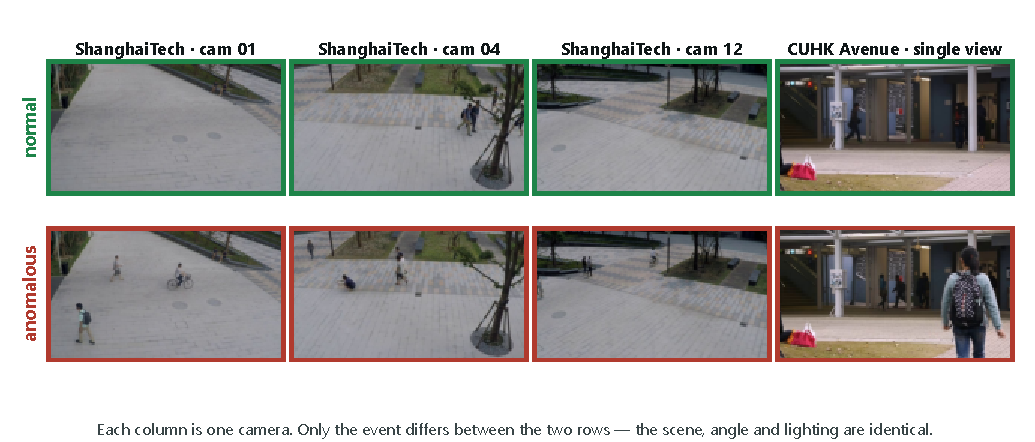
\includegraphics[width=0.9\textwidth]{fig_dataset_samples}
\caption{Normal and anomalous frames from two video benchmarks. Each column is
one fixed camera, so the scene is constant and only the event differs. An empty
walkway and the same walkway with a cyclist look alike but are labelled
oppositely: concept shift in a photograph.}\label{fig:samples}
\end{figure*}

\subsection{Evaluation metrics}
\label{sec:metrics}
Anomalies are rare, so accuracy is uninformative, and every measure here is
threshold-free. Let $\mathcal{A}$ and $\mathcal{N}$ be the anomalous and normal
evaluation frames.

\emph{Frame-level AUROC} \cite{fawcett2006roc, bradley1997auc} is the
probability that an anomalous frame scores above a normal one,
\begin{equation}
\mathrm{AUROC}=\frac{1}{|\mathcal{A}||\mathcal{N}|}\sum_{i\in\mathcal{A}}\sum_{j\in\mathcal{N}}
\Big(\mathbf{1}[\tilde{s}_i>\tilde{s}_j]+\tfrac12\mathbf{1}[\tilde{s}_i=\tilde{s}_j]\Big),
\label{eq:auroc}
\end{equation}
so $0.5$ is chance. The \emph{micro} figure pools the frames of all videos into
one ranking; it is the convention on every benchmark and the figure reported
unless stated otherwise. The \emph{macro} figure averages within-video AUROC.
Pooling ranks frames from different cameras against one another, so it is
sensitive to each camera's score level, and the macro figure is not. The
measurement audit uses exactly this difference. On ShanghaiTech and CUHK Avenue
each clip's scores are min--max normalised before pooling, following the
benchmark protocol \cite{liu2018shanghaitech}. On UBnormal, following its
authors' evaluation code, each sampled frame's score is held for the fifteen
frames that follow it.

\emph{Average precision}, the official measure of XD-Violence
\cite{wu2020xdviolence}, is
\begin{equation}
\mathrm{AP}=\int_0^1 \mathrm{P}\,\mathrm{dR},
\label{eq:ap}
\end{equation}
computed over the precision--recall curve as the official code does.

\emph{The context gap} between two texts given to the same frozen pipeline is
\begin{equation}
\Delta(c_1,c_2)=\mathrm{M}\big(\tilde{s}(\cdot\mid c_1)\big)-\mathrm{M}\big(\tilde{s}(\cdot\mid c_2)\big),
\label{eq:gap}
\end{equation}
where $\mathrm{M}$ is AUROC or AP.

\emph{Uncertainty} comes from a paired bootstrap over whole videos, because
frames within a video are strongly correlated: $B=1000$ resamples with a fixed
seed, both conditions scored on the same resample, and the 95\% interval taken
from the 2.5th to the 97.5th percentile. A difference is \emph{significant} when
its interval excludes zero.

\subsection{Phase 2 development rule and freezing}
\label{sec:rule}
Phase~2 changed one thing at a time. Before each step, the condition, the
reference, the predictions and the decision rule were committed to the
repository, and only then was the step scored. A change $x$ was kept over the
current best $b$ only if the paired differences $\Delta_d=M_d(x)-M_d(b)$ over
the four development benchmarks satisfied
\begin{equation}
\#\{\Delta_d>0\}>2,\quad
\#\{\mathrm{CI}_d\subset(0,\infty)\}\ge2,\quad
\#\{\mathrm{CI}_d\subset(-\infty,0)\}=0.
\label{eq:rule}
\end{equation}
In words, a change must help on most benchmarks, clearly on at least two, and
clearly hurt on none. When the round ended, the hashes of the seven files that
define the model were recorded, together with the UBnormal protocol, three
predictions, and a table of the sentence each possible outcome would permit. The
sealed-test code, with gates that refuse to run if a frozen file has changed,
was committed next. Only then was UBnormal downloaded (Fig.~\ref{fig:timeline}).

\begin{figure*}[!t]
\centering
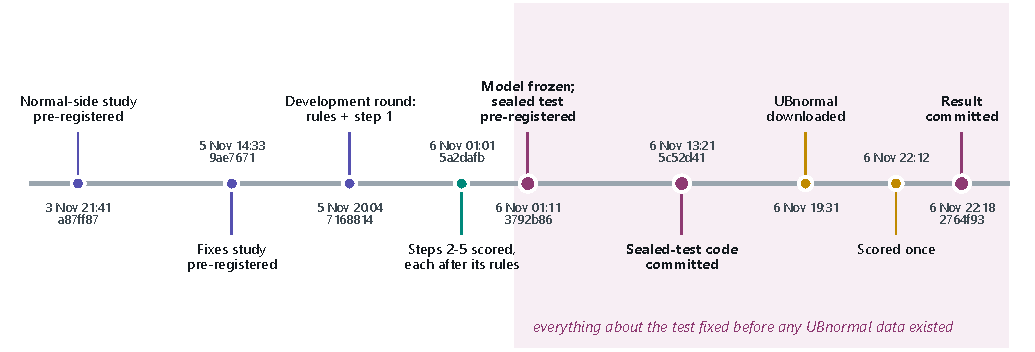
\includegraphics[width=\textwidth]{fig_p2_timeline}
\caption{The Phase~2 evidence chain, with the time and commit of each step (all
times 6~November~2026 unless marked). Everything that determines the sealed
result was committed before the first UBnormal file existed on any of our
machines.}\label{fig:timeline}
\end{figure*}

\subsection{Implementation}
All experiments ran on one NVIDIA A40 under PyTorch 2.3.1. CLIP ViT-L/14
(LAION-2B) and PE-Core-L/14-336 come from \texttt{open\_clip}. Image embeddings
are cached separately from scores, so one encoding pass supports many scoring
hypotheses. Each run records a manifest with the code commit, hardware, library
versions, configuration and label counts, and each run first reproduces the
stored scores of the current best before it scores anything new.

% =====================================================================
\section{Phase 1 Results: What a Scene Description Does}
\label{sec:p1-results}
% =====================================================================

\subsection{Baselines}
On MVTec AD the frozen scorer (M1) reaches $88.5\%$ image AUROC with no training,
against $92.4\%$ for a One-Class SVM \cite{scholkopf2001oneclass} trained on the
same CLIP features. Texture categories average about $99.5\%$ and object
categories about $83.1\%$. Prompt engineering does not help at image level, so
the binding constraint is spatial resolution.

On ShanghaiTech with no description, raw pooled AUROC is $0.519$, close to
chance, while the same scores give $0.707$ once each clip is normalised
(Table~\ref{tbl:video}). The cause is that each camera sits at its own
similarity level (Fig.~\ref{fig:baselines}): what counts as an anomalous
\emph{score} is scene-relative, just as an anomalous \emph{event} is. Smoothing
adds four points from $w=1$ to its optimum $w=31$.

\begin{table}[!t]
\caption{ShanghaiTech, no description: frame-level AUROC by window $w$ under
three pooling conventions. The underlying scores are identical.}
\label{tbl:video}
\centering
\footnotesize
\begin{tabularx}{\columnwidth}{@{}Z c c c c c@{}}
\toprule
\textbf{Pooling} & $w{=}1$ & $5$ & $9$ & $15$ & $31$ \\
\midrule
Micro, raw & 0.493 & 0.502 & 0.508 & 0.513 & 0.519 \\
Macro (per clip) & 0.614 & 0.628 & 0.637 & 0.648 & 0.670 \\
\textbf{Micro, per clip normalised} & \textbf{0.667} & \textbf{0.685} & \textbf{0.691} & \textbf{0.702} & \textbf{0.707} \\
\bottomrule
\end{tabularx}
\end{table}

\begin{figure*}[!t]
\centering
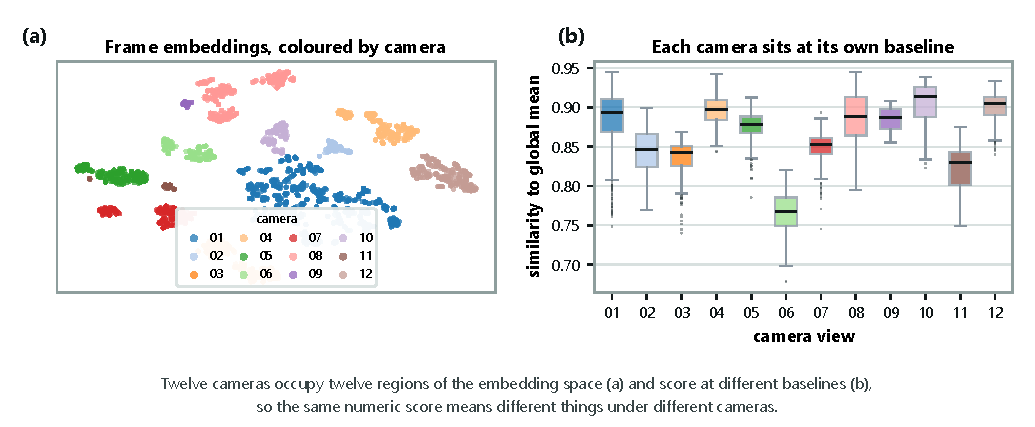
\includegraphics[width=0.9\textwidth]{fig_camera_baselines}
\caption{Why pooling raw scores across cameras fails. (a) Frame embeddings
(t-SNE), coloured by camera: the views occupy distinct regions. (b) Each frame's
similarity to the global mean, per view; the medians differ by more than $0.13$.
No labels are used.}\label{fig:baselines}
\end{figure*}

\subsection{The context sweep: injection point dominates wording}
\label{sec:p1-sweep}
Table~\ref{tbl:sweep} and Fig.~\ref{fig:sweep} give the sweep under two fusion
rules. When the descriptor is added to \emph{both} ensembles, the predicted order
is reversed: matched is the worst condition. When it is added to the
\emph{normal} ensemble only, the predicted signature appears, matched ($0.734$)
$>$ none ($0.707$) $\gg$ mismatched ($0.628$). Fixing the fusion rule moves the
matched-minus-mismatched gap from $-0.029$ to $+0.105$.

\begin{table}[!t]
\caption{Context sweep on ShanghaiTech ($w{=}31$, per clip normalised AUROC).
Only the descriptor and its point of injection vary.}
\label{tbl:sweep}
\centering
\footnotesize
\begin{tabularx}{\columnwidth}{@{}Z c c c c c@{}}
\toprule
\textbf{Fusion} & \textbf{none} & \textbf{gen.} & \textbf{match.} & \textbf{mism.} & \textbf{gap} \\
\midrule
Both ensembles & 0.707 & 0.670 & 0.666 & 0.695 & $-0.029$ \\
\textbf{Normal only} & 0.707 & 0.691 & \textbf{0.734} & 0.628 & $\mathbf{+0.105}$ \\
\midrule
\multicolumn{6}{@{}l}{\emph{Angle between the normal and abnormal prototypes}} \\
Both ensembles & $35.7^\circ$ & $26.3^\circ$ & $26.3^\circ$ & $25.0^\circ$ & \\
Normal only & $35.7^\circ$ & $34.5^\circ$ & $41.9^\circ$ & $37.6^\circ$ & \\
\bottomrule
\end{tabularx}
\end{table}

\begin{figure*}[!t]
\centering
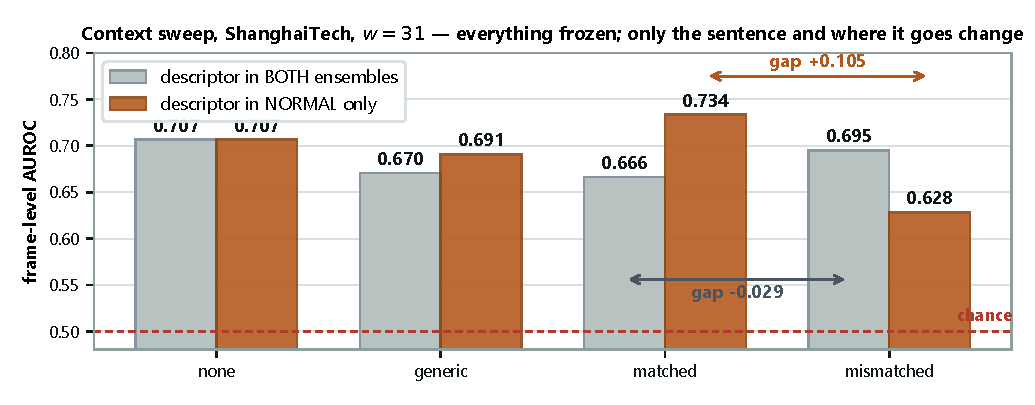
\includegraphics[width=0.9\textwidth]{fig_chart_sweep}
\caption{Table~\ref{tbl:sweep} drawn. The quantity the sweep exists to measure is
the distance between the matched and mismatched bars. Moving the descriptor from
both ensembles to the normal ensemble alone changes it from $-0.029$ to
$+0.105$.}\label{fig:sweep}
\end{figure*}

The mechanism is \emph{prototype dilution}. Each ensemble is mean-pooled, so text
added to both enters both prototypes as a common component. That contracts the
angle between them from $35.7^\circ$ to about $26^\circ$ for every descriptor.
An accurate description is the most harmful of all, because it also drags both
prototypes onto the image embeddings: the mean frame-to-prototype similarity
rises by $+0.067$, against $+0.014$ for the generic text and $-0.017$ for the
mismatched one. The matched-over-none margin ($+0.027$) is positive at every
window but lies inside the split-to-split spread of $\pm0.036$, so we report its
direction only. The mismatched deficit ($-0.105$) is unambiguous: the
description is \emph{load-bearing}.

\subsection{Ablation and single-scene control}
Of five scoring signals, the plain text margin is best ($0.718\pm0.036$ held out
over five clip-level partitions). Adding a kinematic signal (embedding drift,
$0.685$ alone) or scene-centre normality ($0.585$ alone) does not help it. Six
further modifications also failed: local temporal deviation, quadrant scoring,
per-prompt maximum pooling, a domain-specific prompt ensemble ($0.486$), and the
two above.

On single-camera CUHK Avenue the detector transfers ($0.706$ with no
description, against $0.707$ on ShanghaiTech), but the context gap falls to
$+0.020$, and a correct description scores \emph{below} none ($0.677$). Running
the sweep inside each ShanghaiTech view reproduces this
(Table~\ref{tbl:withinview}): the gap shrinks to $+0.033$, with 95\% interval
$[-0.005, +0.070]$, which excludes the pooled $+0.105$. The description mainly
tells the scorer \emph{which} scene it is looking at.

\begin{table}[!t]
\caption{Context gap (matched $-$ mismatched) against the number of scenes the
description must resolve.}
\label{tbl:withinview}
\centering
\footnotesize
\begin{tabularx}{\columnwidth}{@{}Z l c@{}}
\toprule
\textbf{Evaluation} & \textbf{Scenes} & \textbf{Gap} \\
\midrule
CUHK Avenue (single view) & 1 & $+0.020$ \\
ShanghaiTech, mean within a view & 1 each (9 views) & $+0.033$ \\
ShanghaiTech, pooled & 12 & $+0.105$ \\
UCF-Crime, per-video descriptions & ${\sim}290$ & $+0.096$ \\
\bottomrule
\end{tabularx}
\end{table}

\subsection{Per-camera descriptions, by hand and by the model}
If the description identifies the scene, one sentence per camera should beat one
shared sentence, and swapping sentences between cameras should remove the gain
(Table~\ref{tbl:perview}). Descriptions generated by LLaVA with no human input
and no labels reach $0.751$. Both per-camera sets beat every one of the eleven
shuffled assignments. The gain over the shared sentence ($+0.017$) is inside the
noise, so we report its direction only.

\begin{table}[!t]
\caption{Per-camera descriptions on ShanghaiTech ($w{=}31$, per clip normalised).
Shuffled rows give each view another view's sentence (11 rotations).}
\label{tbl:perview}
\centering
\footnotesize
\begin{tabularx}{\columnwidth}{@{}Z c@{}}
\toprule
\textbf{Descriptor} & \textbf{AUROC} \\
\midrule
None & 0.707 \\
One sentence shared by all views & 0.734 \\
Per view, written by hand & 0.749 \\
\textbf{Per view, generated by LLaVA (no human, no labels)} & \textbf{0.751} \\
Per view, hand-written, shuffled (mean / best) & 0.715 / 0.737 \\
Per view, generated, shuffled (mean / best) & 0.707 / 0.722 \\
\bottomrule
\end{tabularx}
\end{table}

\subsection{UCF-Crime under pre-registered predictions}
The protocol and four predictions were committed before any UCF-Crime score was
computed. Each video's description is generated from its first three sampled
frames (Table~\ref{tbl:ucf}). A video's own description beats other videos'
descriptions by $+0.110\ci{+0.069}{+0.157}$, and other videos' descriptions
score \emph{below} none ($0.713$ against $0.756$). P1, which predicted that the
gap would exceed ShanghaiTech's $+0.105$, was refuted ($+0.096$). The claim is
therefore narrowed from ``the benefit scales with scene diversity'' to ``the
benefit requires it''. P2--P4 hold. The per-video figure $0.824\ci{0.756}{0.877}$
is above LAVAD ($80.3$) and AnyAnomaly ($80.7$) in only $72.8\%$ and $67.3\%$ of
resamples, so we call it \emph{comparable} to them, not better.

\begin{table}[!t]
\caption{UCF-Crime (290 videos), raw pooled AUROC, $w{=}5$, with paired
video-level bootstrap intervals.}
\label{tbl:ucf}
\centering
\footnotesize
\begin{tabularx}{\columnwidth}{@{}Z l@{}}
\toprule
\textbf{Descriptor} & \textbf{AUROC} \\
\midrule
None & 0.756 \\
Generic & 0.729 \\
One sentence shared by all videos & 0.813 \\
\textbf{Per video, generated by LLaVA} & $\mathbf{0.824}$ $[0.756, 0.877]$ \\
Per video, shuffled (mean / best of 20) & 0.713 / 0.779 \\
Mismatched (industrial) & 0.727 \\
\midrule
Per video $-$ none & $+0.067$ $[-0.002, +0.153]$ \\
Per video $-$ shared & $+0.011$ $[-0.047, +0.080]$ \\
Per video $-$ other videos' & $+0.110$ $[+0.069, +0.157]$ \\
\bottomrule
\end{tabularx}
\end{table}

\subsection{What the description changes: a measurement audit}
\label{sec:p1-audit}
A pooled gain can come from \emph{re-ranking} frames within a video, or from
\emph{calibration}, which shifts each video's scores as a block. The audit splits
each gap exactly into a \emph{level} part, which a per-video shift alone
reproduces, and a remainder, and measures the change in within-video AUROC
separately. Its decision rule was committed before any audit number existed: a
gap is calibration-dominated if its level share is at least $2/3$ and the
within-video change is at most a third of the gap. Table~\ref{tbl:audit} shows
that the three headline gaps are calibration-dominated ($82$--$87\%$ level). On
ShanghaiTech CLIP's logit scale amplifies the shift: the same gap is $+0.017$ at
$\lambda=1$ and $+0.105$ at $\lambda=100$. A label-free per-video centring rule
does \emph{not} reproduce the description's effect ($0.657$ on ShanghaiTech,
$0.702$ on UCF-Crime). The description puts cameras on one scale; it does not
redefine normality within a scene.

\begin{table}[!t]
\caption{Measurement audit (Phase~1). Level: part of the pooled gap reproduced
by a per-video shift. Within: change in mean within-video AUROC.}
\label{tbl:audit}
\centering
\footnotesize
\begin{tabularx}{\columnwidth}{@{}Z c c c c@{}}
\toprule
\textbf{Comparison} & \textbf{Gap} & \textbf{Share} & \textbf{Within} & \textbf{Verdict} \\
\midrule
ShT, matched $-$ mismatched & $+0.105$ & $0.82$ & $+0.006$ & calibration \\
ShT, per-camera $-$ shuffled & $+0.043$ & $0.34$ & $+0.010$ & mixed \\
UCF, per-video $-$ none & $+0.067$ & $0.83$ & $+0.001$ & calibration \\
UCF, per-video $-$ shuffled & $+0.110$ & $0.87$ & $+0.024$ & calibration \\
\bottomrule
\multicolumn{5}{@{}l}{\scriptsize ShT: ShanghaiTech; UCF: UCF-Crime.}
\end{tabularx}
\end{table}

\subsection{Where it fails: XD-Violence and NWPU Campus}
\label{sec:p1-fail}
On XD-Violence the generated description lowers average precision from $0.624$
to $0.417$ (Table~\ref{tbl:xdnwpu}). In 127 of the 500 violent videos the
violence has already begun within the first three sampled frames, so the caption
that should state what is normal describes the event, and the detector is told
that the anomaly is normal. Removing the description from those 127 videos alone
recovers $66\%$ of the loss. This analysis uses the labels and is exploratory.
On NWPU Campus the per-scene description neither helps nor hurts ($+0.008$),
although a scene's own description beats another scene's ($+0.066$). Any method
that describes a scene from its opening footage inherits this risk, which
motivates Phase~2.

\begin{table}[!t]
\caption{XD-Violence (AP) and NWPU Campus (AUROC), Phase~1 detector; paired
differences with 95\% video-level intervals.}
\label{tbl:xdnwpu}
\centering
\footnotesize
\begin{tabularx}{\columnwidth}{@{}Z l l@{}}
\toprule
\textbf{Description} & \textbf{XD-Violence} & \textbf{NWPU Campus} \\
\midrule
None & 0.624 & 0.659 \\
One shared & 0.582 & 0.648 \\
Generated per video / scene & \textbf{0.417} & 0.667 \\
Generated, shuffled & 0.454 & 0.601 \\
\midrule
Generated $-$ none & $-0.207$ & $+0.008$ \\
 & $[-0.261, -0.155]$ & $[-0.025, +0.043]$ \\
Generated $-$ shuffled & $-0.036$ & $+0.066$ \\
 & $[-0.083, +0.009]$ & $[+0.014, +0.109]$ \\
\bottomrule
\end{tabularx}
\end{table}

Figure~\ref{fig:roc} shows the full curves. On UCF-Crime the description raises
the true-positive rate most at low false-positive rates (about $0.5\to0.7$ at a
false-positive rate of $0.2$). On XD-Violence it lowers precision at almost every
recall, the signature of a uniform shift in score level.

\begin{figure*}[!t]
\centering
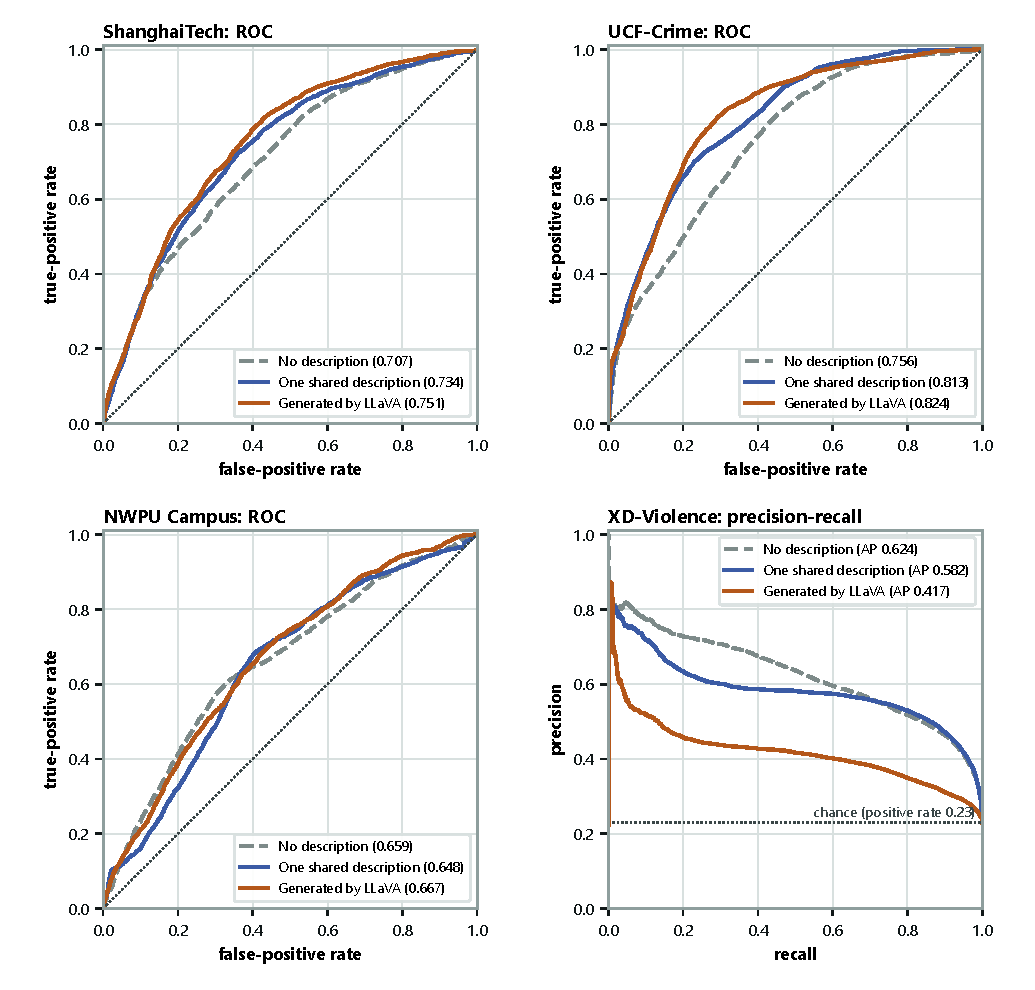
\includegraphics[width=\textwidth,height=0.62\textheight,keepaspectratio]{fig_roc_curves}
\caption{Phase~1: ROC curves (ShanghaiTech, UCF-Crime, NWPU Campus) and the
precision--recall curve (XD-Violence) for the frozen CLIP pipeline with no
description, one shared description, and the description generated by LLaVA.
Areas in the legends are those of Tables~\ref{tbl:perview}, \ref{tbl:ucf}
and~\ref{tbl:xdnwpu}.}\label{fig:roc}
\end{figure*}

% =====================================================================
\section{Phase 2 Results: The Fixed Text Prior}
\label{sec:p2-results}
% =====================================================================

\subsection{From the description-based system to the fixed prior}
Table~\ref{tbl:dev} and Fig.~\ref{fig:progression} follow five configurations
on the same test videos. Replacing CLIP with PE-Core, with the prompts
unchanged, raises UCF-Crime by $+0.091\ci{+0.015}{+0.174}$. It also lowers
XD-Violence by $-0.131\ci{-0.181}{-0.079}$, so a stronger encoder alone is not
the improvement. What it offers is a text space in which the phrases of
Section~\ref{sec:p2-method} work.

\begin{table}[!t]
\caption{The Phase~2 development round on the same test videos: AUROC, and AP
on XD-Violence. The last row was frozen. These figures guided the design and
are exploratory.}
\label{tbl:dev}
\centering
\footnotesize
\setlength{\tabcolsep}{3pt}
\begin{tabularx}{\columnwidth}{@{}Z c c c c@{}}
\toprule
\textbf{Configuration} & \textbf{ShT} & \textbf{UCF} & \textbf{XD} & \textbf{NWPU} \\
\midrule
ViT-L/14, base prompts & 0.707 & 0.756 & 0.624 & 0.659 \\
ViT-L/14 + LLaVA description & 0.751 & 0.824 & 0.417 & 0.667 \\
PE-Core, base prompts & 0.666 & 0.847 & 0.494 & 0.617 \\
PE-Core + calm phrases (C) & 0.757 & 0.817 & 0.635 & 0.669 \\
\textbf{PE-Core + C + bank (B)} & \textbf{0.783} & \textbf{0.856} & \textbf{0.722} & 0.639 \\
\bottomrule
\multicolumn{5}{@{}l}{\scriptsize ShT: ShanghaiTech; UCF: UCF-Crime; XD: XD-Violence; NWPU: NWPU Campus.}
\end{tabularx}
\end{table}

\begin{figure*}[!t]
\centering
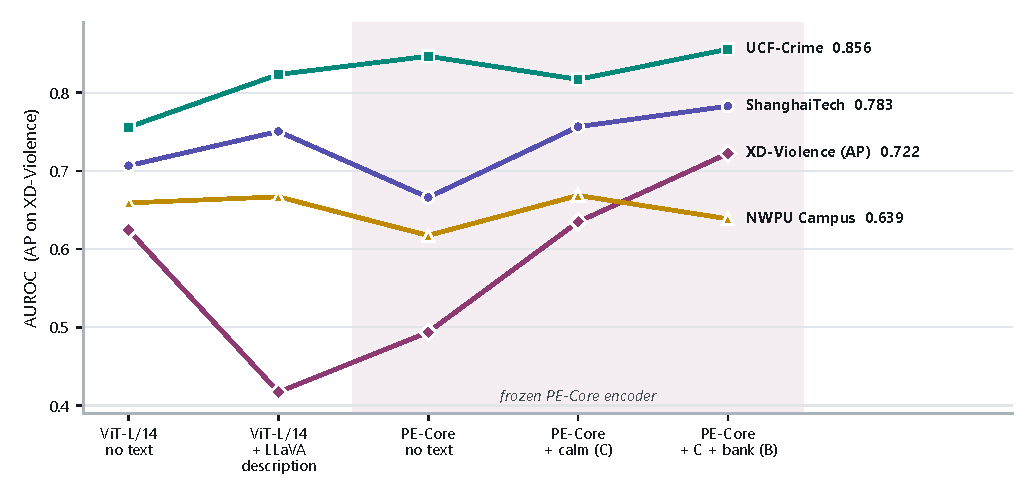
\includegraphics[width=0.85\textwidth]{fig_p2_progression}
\caption{Table~\ref{tbl:dev} as a slope chart. Changing the encoder alone helps
only UCF-Crime. The calm phrases and the bank then recover and exceed the
Phase~1 system on three of four benchmarks, most strongly on XD-Violence, where
the description had failed.}\label{fig:progression}
\end{figure*}

\subsection{What each piece of text contributes}
\label{sec:p2-effects}
Table~\ref{tbl:effects} and Fig.~\ref{fig:forest} give every paired effect.
\emph{Calm phrases:} on PE-Core they raise ShanghaiTech, XD-Violence and NWPU
Campus significantly and leave UCF-Crime within noise, which passes the rule of
Equation~\eqref{eq:rule}. A second wording sharing no phrase also passes, so the
direction does not depend on the words. \emph{Encoder dependence:} the same
phrases do nothing measurable on CLIP ViT-L/14. A text prior is therefore a
property of the words in a particular embedding space, not of the words alone.
\emph{The action bank} adds significantly on UCF-Crime and XD-Violence and also
passes. Against the Phase~1 system, the final model is no worse on any
benchmark and better on XD-Violence by $+0.305$.

\begin{table*}[!t]
\caption{Paired effects with 95\% video-level bootstrap intervals (AUROC; AP on
XD-Violence; micro AUROC on UBnormal). Bold: interval excludes zero. The UBnormal
column comes from the sealed run; a dash means that comparison was not part of
it.}
\label{tbl:effects}
\centering
\footnotesize
\begin{tabularx}{\textwidth}{@{}Z c c c c c@{}}
\toprule
\textbf{Effect} & \textbf{ShanghaiTech} & \textbf{UCF-Crime} & \textbf{XD-Violence} & \textbf{NWPU Campus} & \textbf{UBnormal} \\
\midrule
PE-Core $-$ ViT-L/14, base prompts & $-0.041$ $[-0.085, +0.002]$ & $\mathbf{+0.091}$ $[+0.015, +0.174]$ & $\mathbf{-0.131}$ $[-0.181, -0.079]$ & $-0.042$ $[-0.119, +0.029]$ & --- \\
Calm phrases on PE-Core (C $-$ plain) & $\mathbf{+0.091}$ $[+0.044, +0.142]$ & $-0.030$ $[-0.085, +0.024]$ & $\mathbf{+0.141}$ $[+0.106, +0.170]$ & $\mathbf{+0.051}$ $[+0.008, +0.099]$ & $\mathbf{+0.036}$ $[+0.006, +0.069]$ \\
Second calm wording on PE-Core & $\mathbf{+0.057}$ $[+0.024, +0.094]$ & $-0.012$ $[-0.057, +0.033]$ & $\mathbf{+0.129}$ $[+0.096, +0.157]$ & $\mathbf{+0.052}$ $[+0.014, +0.091]$ & --- \\
Calm phrases on ViT-L/14 & $+0.017$ $[-0.005, +0.040]$ & $-0.021$ $[-0.073, +0.028]$ & $-0.011$ $[-0.036, +0.015]$ & $-0.006$ $[-0.041, +0.030]$ & --- \\
Bank on top of C (B $-$ C) & $+0.026$ $[-0.010, +0.062]$ & $\mathbf{+0.039}$ $[+0.006, +0.074]$ & $\mathbf{+0.088}$ $[+0.067, +0.109]$ & $-0.030$ $[-0.066, +0.001]$ & $\mathbf{+0.060}$ $[+0.016, +0.102]$ \\
Final $-$ Phase 1 description system & $+0.032$ $[-0.006, +0.070]$ & $+0.032$ $[-0.018, +0.087]$ & $\mathbf{+0.305}$ $[+0.255, +0.359]$ & $-0.028$ $[-0.091, +0.031]$ & --- \\
Final $-$ plain PE-Core & --- & --- & --- & --- & $\mathbf{+0.096}$ $[+0.051, +0.142]$ \\
Final $-$ plain ViT-L/14 & --- & --- & --- & --- & $\mathbf{+0.161}$ $[+0.112, +0.215]$ \\
\bottomrule
\end{tabularx}
\end{table*}

\begin{figure*}[!t]
\centering
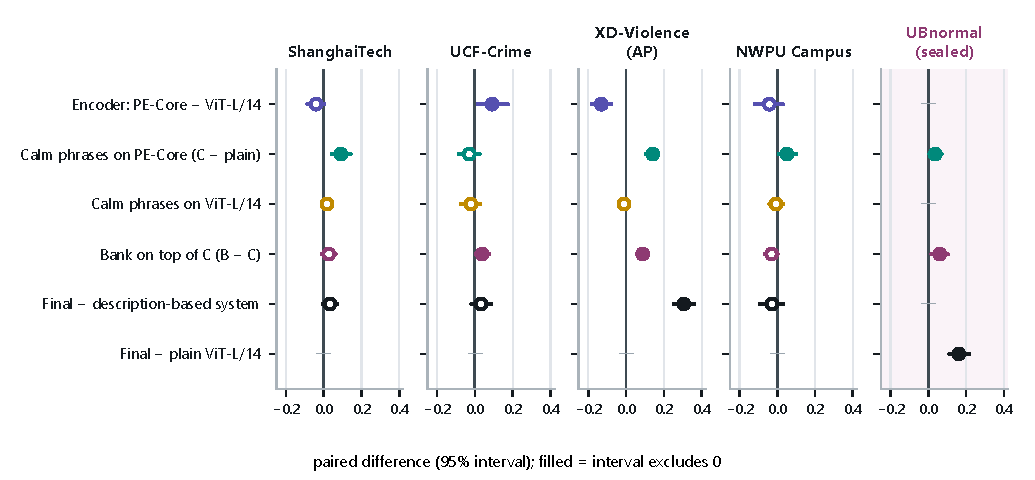
\includegraphics[width=\textwidth]{fig_p2_forest}
\caption{Table~\ref{tbl:effects} drawn: one panel per benchmark, one row per
effect. A filled circle means the 95\% interval excludes zero. The sealed
UBnormal panel (right) shows the same signs as development.}\label{fig:forest}
\end{figure*}

\subsection{Re-ranking on two benchmarks}
The Phase~1 audit, applied to the calm phrases, gives a different picture from
the scene descriptions. On ShanghaiTech their gain is re-ranking-dominated, and
within-video AUROC rises by $+0.166$. On NWPU Campus it is also
re-ranking-dominated (within-video $+0.070$). On XD-Violence, where many videos
contain no anomaly at all, the gain is mainly calibration. On UCF-Crime, where
the phrases did not help ($-0.030$), the audit is mixed. On the two benchmarks
where re-ranking dominates, the calm phrases meet requirement R3 where the
descriptions did not: they change which frames within a video score high.

\subsection{Curves, and what was not kept}
Figure~\ref{fig:devroc} shows the development curves. On ShanghaiTech the final
model lies above both baselines at every false-positive rate. On XD-Violence its
precision is higher at almost every recall.

\begin{figure*}[!t]
\centering
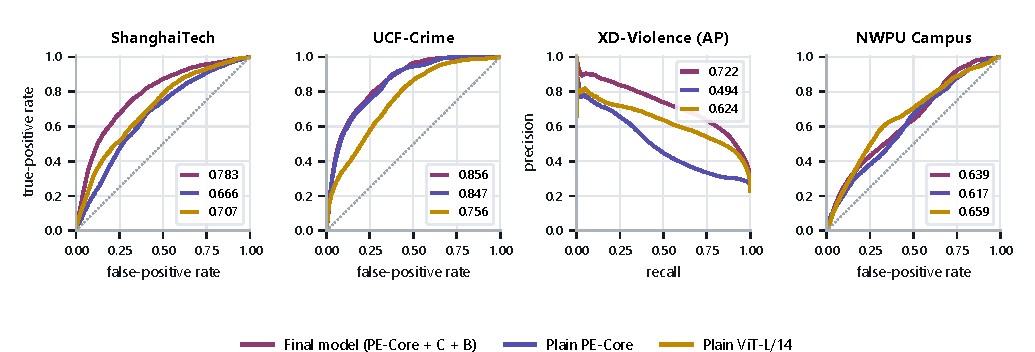
\includegraphics[width=\textwidth]{fig_p2_dev_roc}
\caption{Phase~2: ROC curves on ShanghaiTech, UCF-Crime and NWPU Campus and the
precision--recall curve on XD-Violence, for the final model and the two plain
encoders.}\label{fig:devroc}
\end{figure*}

Table~\ref{tbl:round} lists every development step. Scoring by anomaly type, in
the manner of NOVA \cite{yin2026nova}, raises XD-Violence to $0.769$ but costs
ShanghaiTech $-0.082\ci{-0.138}{-0.025}$. Text sharpened for crime footage
costs accuracy on campus footage. NOVA's visual normal anchor, tested earlier on
PE-Core, lost $-0.037\ci{-0.058}{-0.016}$ on XD-Violence: like the Phase~1
descriptions, a reference taken from each video's own frames is only as normal as
those frames.

\begin{table}[!t]
\caption{Every step of the Phase~2 development round, judged by
Equation~\eqref{eq:rule}.}
\label{tbl:round}
\centering
\footnotesize
\begin{tabularx}{\columnwidth}{@{}l Z Z@{}}
\toprule
\textbf{Step} & \textbf{Change} & \textbf{Outcome} \\
\midrule
1 & Second wording of the calm phrases & passes: calm phrases kept \\
1 & ``Normal scene:'' prefixes on top of C & fails: NWPU $-0.014$ \\
2 & PE-Core and ViT-L/14 averaged & fails: one significant gain \\
3 & Frozen bank of concrete actions (B) & \textbf{passes: kept} \\
3 & Bank scored by anomaly type & fails: ShanghaiTech $-0.082$ \\
3 & Separate templates per side \cite{lee2025flashback} & fails: NWPU $-0.026$ \\
4 & Bank types chosen from each scene & fails: all within noise \\
5 & Novelty against the camera's past & fails: ShT $-0.033$, XD $-0.117$ \\
6 & Per-video baseline subtraction & not run (reason recorded) \\
\bottomrule
\end{tabularx}
\end{table}

% =====================================================================
\section{The Sealed Test on UBnormal}
\label{sec:sealed}
% =====================================================================

UBnormal \cite{acsintoae2022ubnormal} consists of 29 rendered scenes. Its twelve
test anomaly types do not appear in its training split: running, having a
seizure, laying down, shuffling, walking drunk, a person hit by a car, a car
crash, jumping, fire, smoke, jaywalking and driving outside the lane. The bank
names some of these (a car crash, fire, smoke, running, a person lying on the
ground) but not others. UBnormal was named as the held-out benchmark before
development began and was downloaded only after the freeze. Before scoring, the
gates passed: the seven frozen files matched their hashes, the model reproduced
its development scores exactly, and all 211 videos were present. The result is
in Tables~\ref{tbl:sealed} and~\ref{tbl:pred}.

\begin{table}[!t]
\caption{The sealed test on the UBnormal test split, scored once. Micro AUROC
over all 92{,}640 frames is the pre-registered primary measure.}
\label{tbl:sealed}
\centering
\footnotesize
\setlength{\tabcolsep}{3pt}
\begin{tabularx}{\columnwidth}{@{}Z c c c@{}}
\toprule
\textbf{Condition} & \textbf{Micro} & \textbf{95\% interval} & \textbf{Macro} \\
\midrule
\textbf{Final (PE-Core + C + B)} & \textbf{0.747} & \textbf{[0.704, 0.789]} & \textbf{0.906} \\
PE-Core + calm phrases (C) & 0.687 & [0.634, 0.741] & 0.896 \\
Plain PE-Core & 0.651 & [0.599, 0.708] & 0.858 \\
Plain CLIP ViT-L/14 & 0.586 & [0.522, 0.644] & 0.813 \\
\bottomrule
\end{tabularx}
\end{table}

\begin{table}[!t]
\caption{Predictions registered with the freeze, and their outcomes.}
\label{tbl:pred}
\centering
\footnotesize
\begin{tabularx}{\columnwidth}{@{}Z l l@{}}
\toprule
\textbf{Prediction} & \textbf{Measured} & \textbf{Outcome} \\
\midrule
U1: interval of the final model above 0.5 & $[0.704, 0.789]$ & holds \\
U2: final $-$ plain PE-Core above 0 & $+0.096$ & holds \\
U3: final micro AUROC in $[0.60, 0.75]$ & $0.747$ & holds, narrowly \\
\bottomrule
\end{tabularx}
\end{table}

The text prior carried over. The calm phrases add $+0.036\ci{+0.006}{+0.069}$
to plain PE-Core, the bank adds a further $+0.060\ci{+0.016}{+0.102}$, and every
effect has the sign it had in development. In the wording fixed before the test,
the result permits three statements: the model \emph{detects anomalies on an
unseen dataset, without training}; \emph{the calm phrases and bank carried over
to unseen data}; and against plain ViT-L/14 it is \emph{no worse}. The last is
deliberately weak. The rule that would permit ``better'' needs significant gains
on two benchmarks, and a single benchmark cannot meet it, although the interval
of the difference ($+0.161$) lies well above zero.

\paragraph*{Where the score comes from (post hoc)}
The following analyses were not pre-registered. They were run on per-frame
scores exported by a script that first reproduced all four sealed micro AUROCs
exactly. In 20 of the 29 scenes the final model ranks frames better than plain
PE-Core, and the median within-scene AUROC rises from $0.788$ to $0.823$. The
final model also stays above chance in every scene, with a lowest value of
$0.514$ (Fig.~\ref{fig:ubnormal}). Used alone, each of the bank's twelve types
ranks anomalous frames above normal ones better than chance
(Fig.~\ref{fig:types}). \emph{Falling} is strongest ($0.766$), close to
``having a seizure'' and ``laying down''. \emph{Vehicle among pedestrians} is
weakest ($0.542$). The whole bank ($0.744$ under the same unsmoothed conditions)
is close to its best type, so its strength comes from breadth.

\begin{figure*}[!t]
\centering
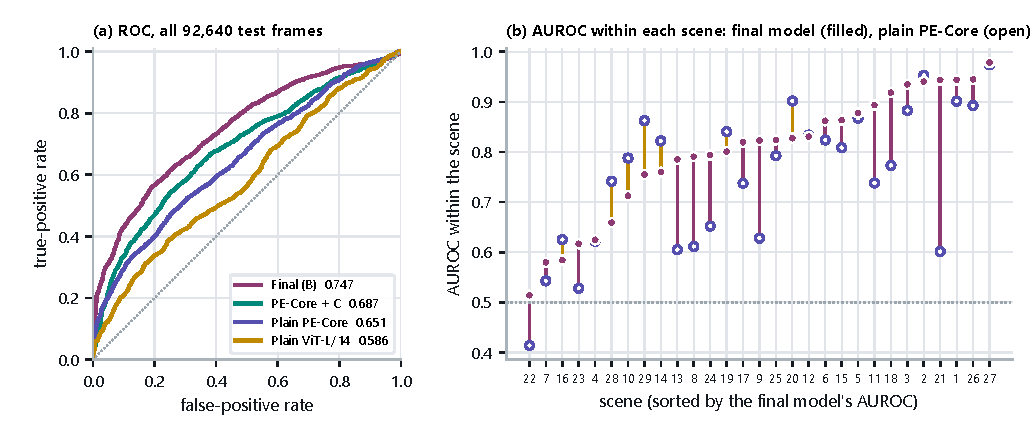
\includegraphics[width=\textwidth]{fig_p2_ubnormal}
\caption{The sealed test in detail. (a) ROC curves of the four conditions over
all test frames; legends give the sealed micro AUROC. (b) AUROC within each
scene for the final model (filled) and plain PE-Core (open). Panel (b) is post
hoc.}\label{fig:ubnormal}
\end{figure*}

\begin{figure*}[!t]
\centering
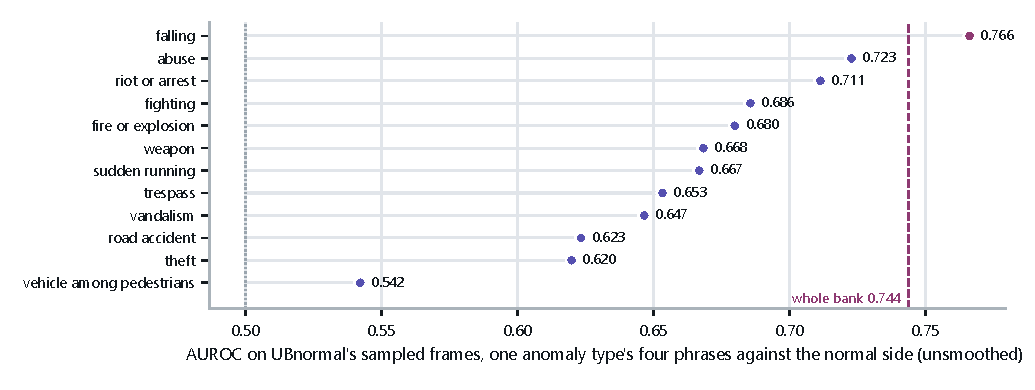
\includegraphics[width=0.85\textwidth]{fig_p2_ubnormal_types}
\caption{Each anomaly type of the bank used alone against the normal side, on
UBnormal's sampled frames without smoothing; the dashed line is the whole bank.
Post hoc and descriptive.}\label{fig:types}
\end{figure*}

\begin{table}[!t]
\caption{Published results on the UBnormal test split (\%). All are micro
frame-level AUROC. $^{a}$From \cite{acsintoae2022ubnormal}, Table~2.
$^{b}$As tabulated in \cite{yang2024anomalyruler}, Table~3.
$^{c}$From \cite{wu2024ovvad}, Table~3.}
\label{tbl:sota-ub}
\centering
\footnotesize
\begin{tabularx}{\columnwidth}{@{}Z l c c@{}}
\toprule
\textbf{Method} & \textbf{Uses from UBnormal} & \textbf{Micro} & \textbf{Macro} \\
\midrule
Georgescu et al.$^{a}$ & normal training videos & 59.3 & 84.9 \\
Georgescu et al.\ + anomalies$^{a}$ & training videos, anomalies & 61.3 & 85.6 \\
Bertasius et al.\ (fine-tuned)$^{a}$ & supervised fine-tuning & 68.5 & 80.3 \\
FPDM$^{b}$ & normal training videos & 62.7 & --- \\
OVVAD$^{c}$ & training videos & 62.94 & --- \\
STG-NF$^{b}$ & normal training videos & 71.8 & --- \\
AnomalyRuler$^{b}$ & a few normal frames, GPT-4 & 71.9 & --- \\
\midrule
\textbf{DA-ZVAD v2 (ours)} & \textbf{nothing} & \textbf{74.7} & \textbf{90.6} \\
\bottomrule
\end{tabularx}
\end{table}

Against published UBnormal results (Table~\ref{tbl:sota-ub}), $74.7$ is above
every micro figure and $90.6$ above every macro figure. STG-NF ($71.8$) and
AnomalyRuler ($71.9$) lie inside our interval $[70.4, 78.9]$, so we say
``above'' and not ``better''. Every published method has also seen UBnormal's
training data, whereas ours has seen nothing of UBnormal.

% =====================================================================
\section{Comparison with Published Methods}
\label{sec:compare}
% =====================================================================

Table~\ref{tbl:sota} and Fig.~\ref{fig:compare} place both phases among
published results. Every external figure was read from its source paper and
recorded with its location before being used.

\begin{table*}[!t]
\caption{Published results on the six video benchmarks (\%): frame-level AUROC;
AP on XD-Violence; micro AUROC on UBnormal. A dash means not reported. Sources:
CUHK Avenue and ShanghaiTech, and UCF-Crime for FPDM, MULDE and AnyAnomaly,
from \cite{anyanomaly2025}, Tables~5--6; $^{\ddagger}$as tabulated in
\cite{zanella2024lavad}; $^{\P}$as tabulated in \cite{cao2023nwpu}, Table~4,
computed over every frame where ours uses every sixteenth; $^{\ast}$as tabulated
in \cite{yin2026nova}, Table~1; $^{\#}$as tabulated in \cite{lee2025flashback},
Table~1; $^{b}$as tabulated in \cite{yang2024anomalyruler}, Table~3; other rows
from each method's own paper. Phase~1 with description: one shared sentence on
Avenue and ShanghaiTech, generated per video on UCF-Crime and XD-Violence and per
scene on NWPU Campus. Our development figures are exploratory; the UBnormal
figures are the sealed result.}
\label{tbl:sota}
\centering
\footnotesize
\begin{tabularx}{\textwidth}{@{}Z c c c c c c@{}}
\toprule
\textbf{Method} & \textbf{CUHK Avenue} & \textbf{ShanghaiTech} & \textbf{UCF-Crime} & \textbf{XD-Violence} & \textbf{NWPU Campus} & \textbf{UBnormal} \\
\midrule
\multicolumn{7}{@{}l}{\emph{Using data from the target benchmark (training, or a few target frames)}} \\
Liu et al.\ \cite{liu2018shanghaitech} & 85.1 & 72.8 & --- & --- & --- & --- \\
MPN \cite{lv2021mpn} & 89.5 & 73.8 & --- & --- & 64.4$^{\P}$ & --- \\
FPDM \cite{yan2023fpdm} & 90.1 & 78.6 & 74.7 & --- & --- & 62.7$^{b}$ \\
MA-PDM \cite{zhou2024mapdm} & 91.3 & 79.2 & --- & --- & --- & --- \\
MULDE \cite{micorek2024mulde} & --- & 81.3 & 78.5 & --- & --- & --- \\
Cao et al., scene-conditioned \cite{cao2023nwpu} & --- & --- & --- & --- & 68.2$^{\P}$ & --- \\
VERA$^{\#}$ \cite{ye2025vera} & --- & --- & --- & 70.54 & --- & --- \\
AnomalyRuler \cite{yang2024anomalyruler} & --- & 85.2 & --- & --- & --- & 71.9$^{b}$ \\
STG-NF$^{b}$ & --- & --- & --- & --- & --- & 71.8 \\
\midrule
\multicolumn{7}{@{}l}{\emph{Training-free: no target data, no gradient updates}} \\
Zero-shot CLIP \cite{radford2021clip} & 62.3 & 60.9 & 53.2$^{\ddagger}$ & 17.8$^{\ddagger}$ & --- & --- \\
Zero-shot ImageBind \cite{girdhar2023imagebind} & 64.5 & 61.3 & 53.7$^{\ddagger}$ & 27.3$^{\ddagger}$ & --- & --- \\
LLaVA-1.5 \cite{liu2023llava} & 67.4 & 59.6 & 72.8$^{\ddagger}$ & 50.3$^{\ddagger}$ & --- & --- \\
Video-ChatGPT \cite{maaz2024videochatgpt} & 76.9 & 69.1 & --- & --- & --- & --- \\
LAVAD \cite{zanella2024lavad} & --- & --- & 80.3$^{\ddagger}$ & 62.0$^{\ddagger}$ & --- & --- \\
AnyAnomaly \cite{anyanomaly2025} & 87.3 & 79.7 & 80.7 & --- & --- & --- \\
EventVAD$^{\ast}$ & --- & --- & 82.03 & 64.04 & --- & --- \\
VADTree$^{\ast}$ & --- & --- & 84.74 & 68.85 & --- & --- \\
PANDA$^{\ast}$ & --- & --- & 84.89 & 70.16 & --- & --- \\
Frozen VLM, yes/no probability \cite{song2026vlmanswer} & --- & --- & 85.3 & 69.0 & --- & --- \\
Flashback-PE \cite{lee2025flashback} & --- & --- & 87.3 & 75.1 & --- & --- \\
ASK-Hint \cite{zou2026askhint} & --- & --- & 89.8 & --- & --- & --- \\
NOVA \cite{yin2026nova} & --- & --- & 89.9 & 84.8 & --- & --- \\
\midrule
DA-ZVAD Phase 1, no description (ours) & 70.6 & 70.7 & 75.6 & 62.4 & 65.9 & 58.6 \\
DA-ZVAD Phase 1, with description (ours) & 67.7 & 73.4 & 82.4 & 41.7 & 66.7 & --- \\
\textbf{DA-ZVAD v2, final (ours)} & --- & \textbf{78.3} & \textbf{85.6} & \textbf{72.2} & \textbf{63.9} & \textbf{74.7} \\
\bottomrule
\end{tabularx}
\end{table*}

\begin{figure*}[!t]
\centering
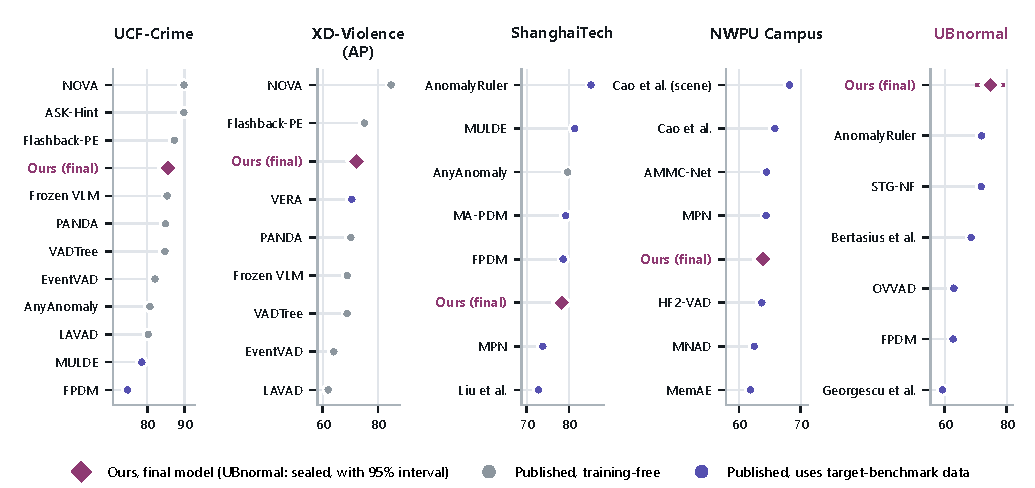
\includegraphics[width=\textwidth]{fig_p2_comparison}
\caption{The final model against published results, one panel per benchmark,
sorted by score. Diamonds: the final model, with its 95\% interval on UBnormal.
Grey: published training-free methods. Blue: published methods that use data
from the target benchmark.}\label{fig:compare}
\end{figure*}

Among training-free methods the final model is behind NOVA, ASK-Hint and
Flashback-PE on UCF-Crime and behind NOVA and Flashback-PE on XD-Violence, and
ahead of the rest. On ShanghaiTech it lies among the one-class methods that train
on that benchmark, and on NWPU Campus inside the range of the trained methods.
Three cautions apply. Our development intervals span several points, so gaps of
one or two points there are not differences. The development figures are
exploratory. And the strongest methods are informed differently: NOVA writes
prompt banks for each anomaly class with dataset-specific guidance
\cite{yin2026nova}, Flashback retrieves from a memory of a million generated
captions \cite{lee2025flashback}, and ASK-Hint queries a large video-language
model \cite{zou2026askhint}. We are not aware that any of them has been
evaluated on a benchmark held out from its own design, which is the setting of
our UBnormal figure. The Phase~1 rows show the progression: plain CLIP reaches
$58.6$ on UBnormal, and the fixed prior on PE-Core reaches $74.7$.

% =====================================================================
\section{Discussion}
\label{sec:discussion}
% =====================================================================

\paragraph*{What changed between the phases}
The Phase~1 description told the detector which scene it was looking at, and it
mostly moved whole videos up or down. The Phase~2 prior tells it what ordinary
and alarming footage look like in general. On two of the four development
benchmarks it mainly reorders frames within a video. It also removes the
dependence on a camera's opening frames, the cause of the XD-Violence failure,
and the resulting model is simpler: no captioning model, no per-camera step, and
one encoder pass per sampled frame.

\paragraph*{Why might calm phrases help?}
Phrases such as ``a normal scene'' sit close to everything, so the normal
prototype barely separates quiet frames from busy ones. Phrases about empty
places and still people point it toward low motion and few people, and
surveillance anomalies are mostly the opposite. That they help PE-Core and not
CLIP suggests that PE-Core's text space represents such \emph{states} of a scene
more distinctly. This is a hypothesis: the experiments show the dependence on the
encoder but not its cause.

\paragraph*{Why did NWPU Campus not improve?}
NWPU Campus contains anomalies that are anomalous only in particular scenes,
such as cycling on a footpath \cite{cao2023nwpu}, and a fixed list cannot know
which scene forbids what. This is the cost of requirement R1. The Phase~1
scene descriptions, which did not help there either, did not pay it back.

\subsection{Threats to validity}
\begin{itemize}
  \item \emph{Development reuse.} The four development benchmarks were used to
        choose the design, and their intervals are not corrected for multiple
        comparisons. Only the UBnormal figure is a test.
  \item \emph{An informed bank.} A large language model that knew the
        development benchmarks' anomaly types wrote the bank. The UBnormal paper,
        which lists its test anomaly types, had been read (3~November~2026)
        before the bank was written (5~November~2026). No UBnormal video or label
        was seen before scoring, but the overlap between bank and list may owe
        something to that reading.
  \item \emph{One synthetic test.} UBnormal is computer-generated, and a single
        benchmark is a single test.
  \item \emph{Narrow prediction.} U3 held by $0.003$; its range, set before any
        UBnormal data existed, was conservative rather than tuned.
  \item \emph{Pooled metric and logit scale.} Pooled, per-clip-normalised AUROC
        depends on the softmax temperature (the ShanghaiTech gap is $+0.017$ at
        $\lambda=1$ and $+0.105$ at $\lambda=100$).
\end{itemize}

\subsection{Limitations and future work}
Both models score whole frames, so anomalies too small or too brief to change a
frame's embedding are invisible. CLIP's centre crop also hides the left and right
edges of wide frames. Patch-level scoring against the encoder's spatial tokens
\cite{jeong2023winclip, zhou2024anomalyclip} is the next step. A frozen video
encoder would address anomalies defined by motion. A fixed text prior cannot
express scene-dependent rules. A second held-out benchmark with such rules, and
real rather than rendered footage, are the tests that remain. The calm phrases'
dependence on the encoder should be examined across more encoders, and the bank
should be rewritten by a model that has not seen any of the benchmarks. The
explanation stage of Phase~1 has not been evaluated against human judgement.

% =====================================================================
\section{Conclusion}
\label{sec:conclusion}
% =====================================================================

This report asked what the text in a training-free video anomaly detector should
say. A description of each camera's scene, written by a frozen model from the
camera's first frames, is load-bearing: a wrong one costs accuracy. However, its
benefit depends on where it enters the prompts and on there being several scenes
to tell apart, it mostly calibrates cameras against one another, and it fails
when the opening footage already shows the event. One fixed set of 59 phrases,
written once and used unchanged on every camera, does better. It matches the
description-based system on three of four development benchmarks and is far
better on the one where per-camera text failed. It was developed under committed
rules and frozen before a fifth benchmark was obtained, and it then reached
$0.747$ AUROC on UBnormal, $+0.096$ above the same encoder alone, with every
pre-registered prediction holding. A training-free detector need not be told
where it is; it can be told, once, what calm footage looks like and what goes
wrong.

\section*{Acknowledgment}
The authors thank the Department of Computer Science and Engineering, National
Institute of Technology Calicut, for access to its GPU server.
% CONFIRM THE WORDING WITH THE SUPERVISORS BEFORE SUBMISSION.
Claude (Anthropic) was used to assist with code, analysis and the drafting of
text, and a large language model generated the abnormal phrase bank
(Section~\ref{sec:p2-method}); the authors reviewed all content and take full
responsibility for it.

\bibliographystyle{IEEEtran}
\bibliography{references}

\end{document}
